\chapter{Die Wirkung von Caspr2 am Axon und der Synapse}
\textbf{Johanna Hoppe}

Bei der beschriebenen Form der Erregungsleitung entlang des Axons
spielen neben den spannungsgesteuerten Ionenkanälen (vgl. Kapitel 2.1.2) auch weitere Proteine eine entscheidende Rolle.

Bereits 1999 wurde das Protein Contactin-associated
protein~2 (Caspr2) in den angrenzenden Bereichen der axonalen Schnürringe, den
juxtaparanodalen Bereichen,
beschrieben\footcite{Poliak1999} und seitdem weiter erforscht. Caspr2
ist ein Typ-I-Transmembranprotein, also ein integrales Protein, welches
die Zellmembran nur einmal durchquert, und gehört zur
Neurexin-Superfamilie. Diese ist eine Gruppe von
Transmembranmolekülen, die Zell-Zell-Kontakte vermitteln und
spezialisierte membranöse Domänen
erzeugen. Caspr2 wiest eine charakteristische Domänenstruktur auf, die in Abbildung 3.2 Teil B dargestellt ist. Dazu gehören unter anderem die Discoidin-Domäne (F58C) und die Laminin-Domänen (L1--L4), welche in Kapitel 6 der Arbeit erneut aufgegriffen werden. \footcites{HaklaiTopper2010}{CellSignaling2026} 

Caspr2 ist am myelinisierten Axon unter anderem mit Contactin2
Bestandteil eines Proteinkomplexes, welcher in Abbildung \ref{fig:cmyelin} dargestellt
ist. Dieser lokalisiert und verankert spannungsgesteuerte
Kalium-Ionenkanäle des Typs Kv1 in der Axonmembran. Dabei interagiert
Caspr2 extrazellulär mit Contactin2, welches wie Caspr2 als
Zelladhäsionsprotein wirkt. Dadurch trägt der Komplex entscheidend zur
räumlichen Organisation der myelinisierten Axonmembran und zur
Aufrechterhaltung einer effizienten saltatorischen
Erregungsweiterleitung bei. (siehe Kapitel~2.1.2) Eine Störung dieser
Interaktion kann die korrekte Clusterbildung und somit die Funktion der
Kv1-Kanäle beeinträchtigen und zu neurologischen Symptomen ,wie in
Kapitel~4.1 beschrieben wird,
führen.\footcite{VanSonderenNatRev2016}
\clearpage
% ── Abbildung 5 ausgelassen ──────────────────────────────────
% Abbildung 5: Caspr2 am myelinisierten Axon - BILD MIT BESSERER QUALI VON SELL EINFÜGEN
% Quelle: \cite{VanSonderenNatRev2016}
% ─────────────────────────────────────────────────────────────
\begin{figure}[h] % [h] versucht, das Bild hier zu platzieren (hier), [t] für oben, [b] für unten
	\centering % Zentriert das Bild horizontal
	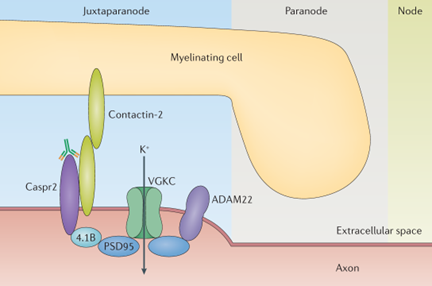
\includegraphics[width=0.91\textwidth]{abbildungen/caspr2myelinWCA.png} % Lädt das Bild, skaliert es auf 80% der Textbreite
	\caption{  Caspr2 am myelinisierten Axon \parencite{SonderenBild2017}} % Die Bildunterschrift
	\label{fig:cmyelin} % Ein Label für Querverweise (z.B. "siehe Abbildung \ref{fig:beispielbild}")
\end{figure}

Zudem ist bekannt, dass Caspr2 während der Embryonalentwicklung
bedeutsam ist und dort für die korrekte Verzweigung der Dendriten, die
Ausbildung dendritischer Spines und das Axonwachstum mitverantwortlich
ist. Fehlt Caspr2 durch eine genetische Veränderung, kann die
Entwicklung der Nervenzellen beeinträchtigt sein. Eine Caspr2-Mutation
wird beispielsweise auch mit Erkrankungen wie der
Autismus-Spektrum-Störung oder Aufmerksamkeits-/Hyperaktivitätsstörung
(ADHS) in Verbindung
gebracht.\footcite{Canali2018}

Neuere Studien zeigen, dass Caspr2 nicht nur am Axon lokalisiert ist,
sondern auch an Synapsen vorkommt, was bisher jedoch deutlich weniger
erforscht ist. Kv1-Kanäle sind bereits sicher an den präsynaptischen
Membranen bekannt und sind dort an der Freisetzung von
Neurotransmittern beteiligt (siehe Kapitel~2.1.2). Bereits 2008 konnten
Caspr2 und Contactin-2 biochemisch an synaptischen Membranen
nachgewiesen werden.\footcite{Bakkaloglu2008}
In einer weiteren Studie aus dem Jahr 2015 wurde mithilfe von
Immunfärbungen eine Überlappung von Caspr2 mit synaptischen Markern
erregender und hemmender Synapsen gezeigt. Dabei wurden die Marker
VGlut für exzitatorische, und Gad65 für inhibitorische Synapsen,
verwendet. Diese gelten als spezifische Markerproteine für den
jeweiligen Synapsentyp. Unter anderem durch solche Ergebnisse wird davon ausgegangen, dass Caspr2 auch an präsynaptischen Membranen
vorliegt.\footcite{Pinatel2015}

Die Funktion von Caspr2 an der Synapse ist bislang nicht vollständig
geklärt, ähnelt jedoch vermutlich der am Axon. Caspr2 bildet auch hier
einen Protein-Komplex mit weiteren Molekülen wie Contactin-2. Wie
dieser genau aufgebaut ist, ist jedoch noch unklar. Angenommen wird,
dass dieser Komplex analog zum myelinisierten Axon die Kv1-Kanäle
stabilisiert und lokalisiert. Darüber hinaus könnte der
Caspr2-Contactin-2-Komplex an der Organisation synaptischer Strukturen
beteiligt sein, indem er die Verbindung von Prä- und Postsynapse
stabilisiert. Die Anordnung des Proteinkomplexes sowie die Organisation
der einzelnen Domänen von Caspr2 ist wahrscheinlich eine andere als am
Axon, da es sich hier um andere Zellbereiche handelt. Weiterhin ist zu
beachten, dass der synaptische Spalt kleiner ist als der extrazelluläre
Raum zwischen Axon und Gliazelle. Entsprechend existieren
unterschiedliche Hypothesen zur Organisation und Funktion von Caspr2 an
der Synapse.\footcite{Canali2018} Teil~C der Abbildung \ref{fig:domänenc}  veranschaulicht zwei mögliche Anordnungen des Proteins an der Synapse:
zum einen eine vertikale Orientierung, die das Protein annehmen könnte,
sowie eine mögliche horizontale Orientierung der Domänen. Je nachdem,
wie das Protein ausgerichtet ist, wird seine Funktion unterschiedlich
beeinflusst, da beispielsweise andere Interaktionen mit weiteren
Proteinen möglich sind.\footcite{Canali2018}
% ── Abbildung 6 ausgelassen ──────────────────────────────────
% Abbildung 6: Domänenorganisation von Caspr2 A ABSCHNEIDEN
% Quelle: \cite{Canali2018}
% ─────────────────────────────────────────────────────────────
\begin{figure}[h] % [h] versucht, das Bild hier zu platzieren (hier), [t] für oben, [b] für unten
	\centering % Zentriert das Bild horizontal
	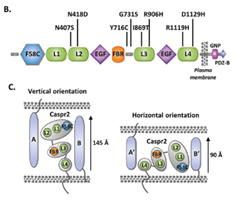
\includegraphics[width=0.91\textwidth]{abbildungen/Domänencaspr2WCA.png} % Lädt das Bild, skaliert es auf 80% der Textbreite
	\caption{Domänenorganisation von Caspr2 \parencite{CanaliBild2018}} % Die Bildunterschrift
	\label{fig:domänenc} % Ein Label für Querverweise (z.B. "siehe Abbildung \ref{fig:beispielbild}")
\end{figure}